\begin{center}
	{\textbf{CARGA Y DESCARGA DE UN CONDENSADOR}}
\end{center}
\section{Objetivo}
Investigar la curva de tensión de carga de un condensador, así como, los factores que afectan el índice carga/descarga y qué efecto tienen estos factores en el índice.
\section{Materiales}
\begin{itemize}
	\item Fuente de alimentación 0 - 12$V$/6$V$ DC/AC.
	\item Interruptor.
	\item Conmutador.
	\item Resistencia de 10 y 47 $K$ \textohm.
	\item Condensador electrolítico de 47 y 470$ \mu $ $F$, bipolar.
	\item Alambre en bloque de conexión.
	\item Cables de conexión rojo y azul.
	\item Multímetro.
	\item Cronometro.
	\item Tablero de conexión.  
\end{itemize}
\section{Fundamento Teórico}
El alumno vendrá estudiando los siguientes prototipos:
\begin{itemize}
	\item Carga y descarga de un condensador.
\end{itemize}
\section{Montaje}
\begin{itemize}
	\renewcommand{\theenumi}{\Alph{enumi}}
	\item \textbf{ Primer experimento:} Monte el circuito como se muestra en la figura 1 y 2. Selecciona el multímetro a escala de 10 $V$ y ponga la llave selectora en posición 1.
	\begin{figure}[h]
		\centering
		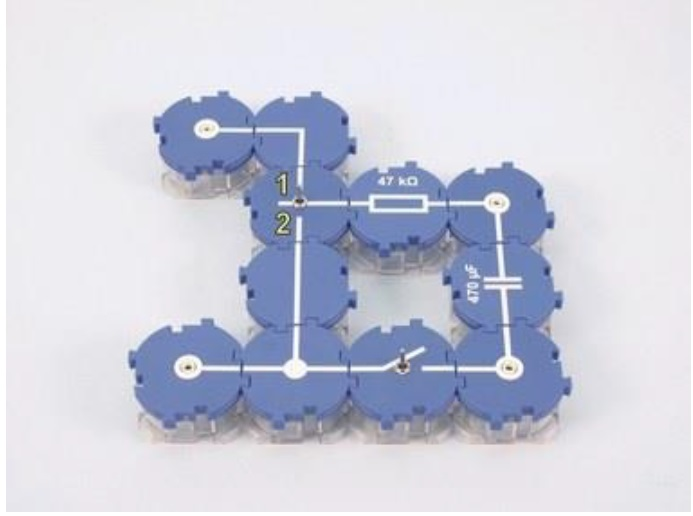
\includegraphics[width=5cm, height= 5cm]{imagenes/figura1}
		\caption{Primer circuito a montar}
	\end{figure}
	\begin{figure}[h]
		\centering
		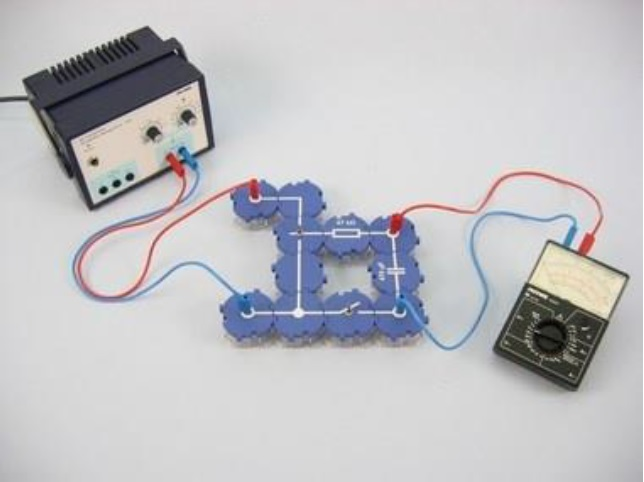
\includegraphics[width=5cm, height=5cm]{imagenes/figura2}
		\caption{Primer circuito siendo medido por un multímetro}
	\end{figure}
	\\
	\\
	\item \textbf{Segundo experimento:} Monte el circuito como se muestra  en la figura 3.
	\begin{figure}[h]
		\centering
		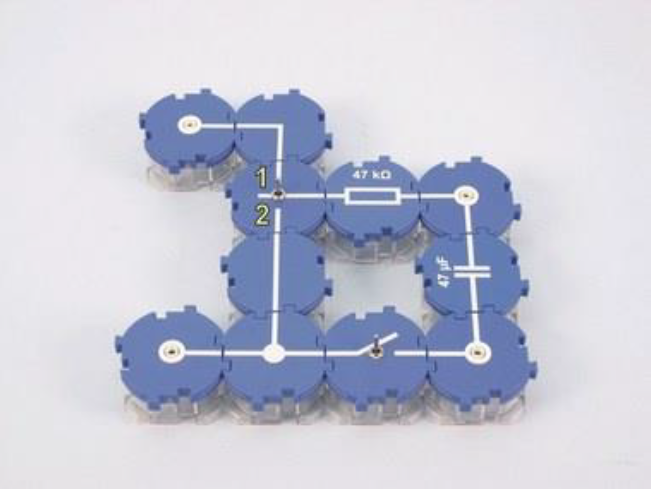
\includegraphics[width=5cm, height=5cm]{imagenes/figura3}
		\caption{Segundo circuito a montar}
	\end{figure}
\end{itemize}

\section{Procedimiento}
\textbf{Del primer experimento:}
\begin{itemize}
	\item Monte el experimento tal como se muestra en la figura  1. El interruptor debería estar en la posición de apagado y el conmutador se debería pulsa t a la posición 1. Seleccione ene voltímetro el rango de medición de 10 $V$.
	\item Encienda la fuente de alimentación y fije la tensión directa a 10 $V$.
	\item Cargue el circuito pulsando interruptor a la posición encendido y observe el voltímetro. Anote sus observaciones en (1).
	\item Descargue el circuito pulsando el conmutador a la posición 2. Observe el voltímetro  una vez más y anote su observación en (2).
	\item Cortocircuite el condensador por unos segundos usando un cable de conexión de 25cm. Retire el cortocircuito cuando la  tensión del condensador sea $U_{c}$ = 0 $V$.
	\item Pulse el conmutador a la posición 1, iniciando en 0 $V$. Mida la tensión $U_{c}$ del condensador en intervalos de 10 segundos. Anote en la tabla 1.
\end{itemize}
\textbf{NOTA:} La toma de medidas requiere  una gran concentración y probablemente un poco de práctica. Si falla la primera serie de medidas, cortocircuite brevemente el condensador y repita las mediciones.
\begin{itemize}
	\item Pulse el conmutador a la posición 2 y tome las medidas de la tensión del condensador en intervalos de 10 segundos. Registre los valores en la tabla 1.
	\item Interrumpa la carga del circuito colocando el interruptor en la posición abierta.
\end{itemize}
\textbf{Del segundo experimento:}
\begin{itemize}
	\item Ponga el conmutador en la posición 1. Cargue el circuito y mida el tiempo que le toma al condensador llegar a $U_{c}$= 6 $V$.
	\item Abra el interruptor. Descargue el condensador y reemplace con el condensador de 47$\mu$$F$.
	\item Cargue el circuito y una vez más mida el tiempo que toma en llegar a $U_{c}$=6$V$. Anote el tiempo en la tabla 2.
	\item Reemplace la resistencia de 47$K$\textohm con una de 10$K$\textohm y repita las mediciones.
	\item Reemplace el condensador de 47$?\mu$$F$ con uno de 470$\mu F$ y repita las mediciones.
	\item Apague la fuente de alimentación.
\end{itemize}
\section{Observaciones y resultados de las mediciones}

